\documentclass[brown]{beamer}
\usepackage{beamerthemesidebar}
%\usepackage{pgf}
\usepackage{graphicx}
% Use some nice templates

\beamertemplatesolidbackgroundcolor{white}
\beamertemplateshadingbackground{white}{structure!15}
\beamertemplatetransparentcovereddynamic
\beamertemplatenumberedballsectiontoc

% the debian logo
\pgfdeclareimage[height=1cm]{logo}{openlogo-nd-100}
\logo{\pgfuseimage{logo}}

\title[d-i internals]{debian-installer internals}
% \subtitle{An introduction to the inner working of debian-installer}
\author[G. Steinlin]{Gaudenz Steinlin}
\date{\today}
\pgfdeclareimage[height=3cm]{titlegraph}{openlogo-nd-100}
\titlegraphic{
\pgfuseimage{titlegraph}

}


\begin{document}

\frame[plain]{
  \titlepage
  \begin{center}
    \tiny This talk is licensed under the terms of the GNU General Public License. \\
    \copyright\ 2004 Gaudenz Steinlin \textless gaudenz@soziologie.ch\textgreater
  \end{center}
}

\section*{Outline}
\frame{
  \frametitle{Outline}
  \tableofcontents
  
  Special thanks go to Thorsten Sauter and Sebastian Ley.
}

\section[Past, Present and Future]{Past, Present and Future - a short introduction}
\frame[label=past]{
  \frametitle{The past}
  \begin{block}<+->{boot-floppies}
    \begin{itemize}
    \item Used with Woody
    \item Monolithic design
    \item Hard to maintain
    \end{itemize}
  \end{block}
  \begin{block}<+->{debian-installer}
    \begin{itemize}
    \item Developement nearly stalled for some time
    \item Huge developement acceleration during the last year
    \item Not used in any Debian release so far
    \end{itemize}
  \end{block}
}
\frame[label=present]{
  \frametitle{The present}
  \begin{itemize}
  \item d-i is nearly release quality (rc1 underway)
  \item Porting to most architectures almost done
  \item Bug squashing and fine tuning for release
  \item No big changes anymore before releasing Sarge
  \end{itemize}
}
\frame[label=future]{
  \frametitle{The future}
  \begin{itemize}
  \item Well done graphical front-end
  \item Custom installers made easy
  \item Automated or unattended installs
  \item Install without reboot?
  \item ...
  \item (The modular design makes additions easier.)
  \end{itemize}
}

\section[Walkthrough]{Walkthrough the installation process}
\frame[label=boot]{
  \frametitle{Stage 0: booting}
  \framesubtitle{\textbf{Goal: Get the installer running}}

  \only<1>{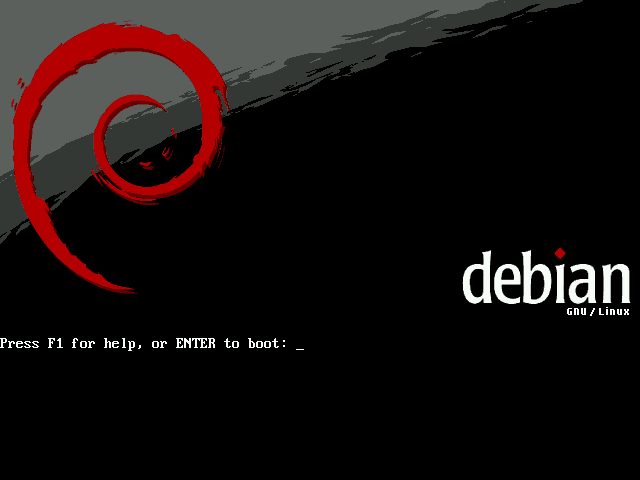
\includegraphics[height=6cm]{000-boot}}
  \only<2-3>{
    \begin{block}<2->{Standard path:}
      \begin{enumerate}
      \item Booting of the computer by the BIOS, OpenFirmware, ...
      \item Loading of the boot-loader from CD-ROM
      \item Loading of the kernel and initial ramdisk
      \item Starting the kernel
      \end{enumerate}
    \end{block}

    \begin{block}<3->{Additional paths:}
      \begin{itemize}
      \item Booting from another OS (loadlin, BootX)
      \item Network Boot (PXE, TFTP, ...)
      \item Loading of kernel and initial ramdisk from floppy
      \item Booting from USB memory stick
      \end{itemize}
    \end{block}
  }
}  

\frame[label=initrd]{
  \frametitle{Stage 1a: initial ramdisk}
  \framesubtitle{\textbf{Goal: setup access to additional components}}
  \only<1>{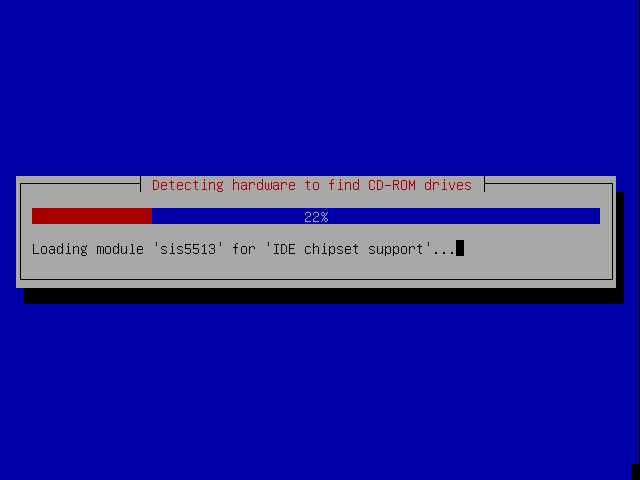
\includegraphics[height=6cm]{009-cd-detect}}
  \only<2->{
    \begin{enumerate}
    \item<2-> Setup shm filesystem, copy initrd content and pivot\_root into it
    \item<3-> Choose installation language, country and keyboard
    \item<4-> First hardware detection
    \item<5-> Different paths depending on installation medium
      \begin{itemize}
      \item Network configuration on netboot and floppy installs
      \item CD drive detection on CD-ROM installs
      \item Detection of other medias containing installer components
      \end{itemize}
    \item<6-> Load additional installer components (from cdrom, network or iso-image)
    \end{enumerate}
  }
}  
\frame[label=stage1b]{
  \frametitle{Stage 1b: after loading additional components}
  \framesubtitle{\textbf{Goal: Install the base-system and make it bootable}}
%  \only<1>{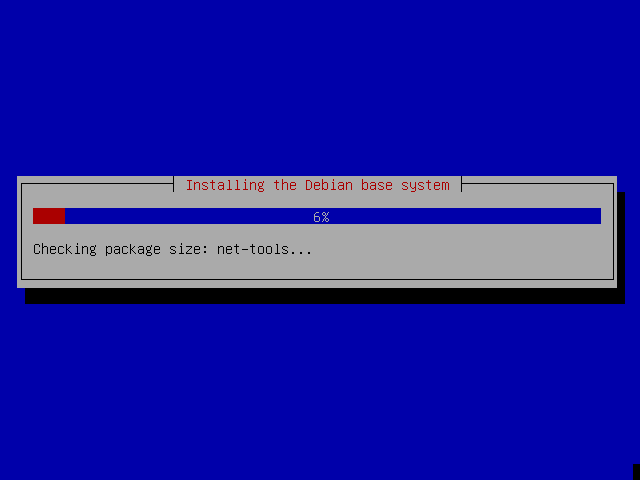
\includegraphics[height=6cm]{093-base-install}}
  \only<1>{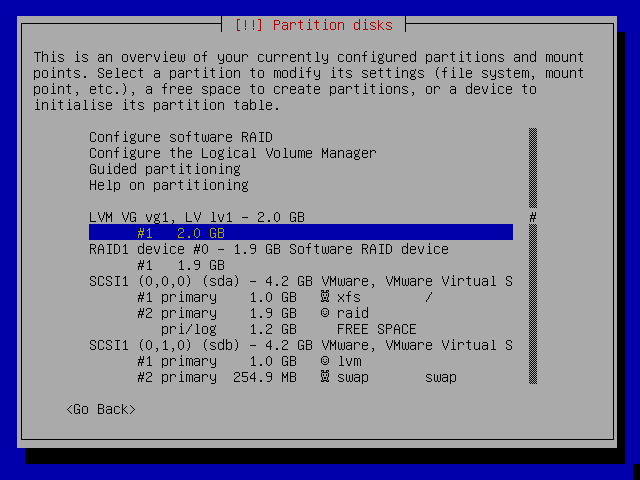
\includegraphics[height=6cm]{092-lvm-result}}
  \only<2->{
  \begin{enumerate}
  \item<2-> Partition disks and assign mount points
  \item<3-> Install base system (from cdrom, network or iso-image)
  \item<4-> Install a few additional packages and kernel
  \item<5-> Install boot loader
  \item<6-> Save settings and logs for 2nd stage and reboot
  \end{enumerate}
}
}  
\frame[label=base-config]{
  \frametitle{Stage 2: base-config}
  \framesubtitle{\textbf{Goal: Install additional packages and configure the system}}
  \only<1>{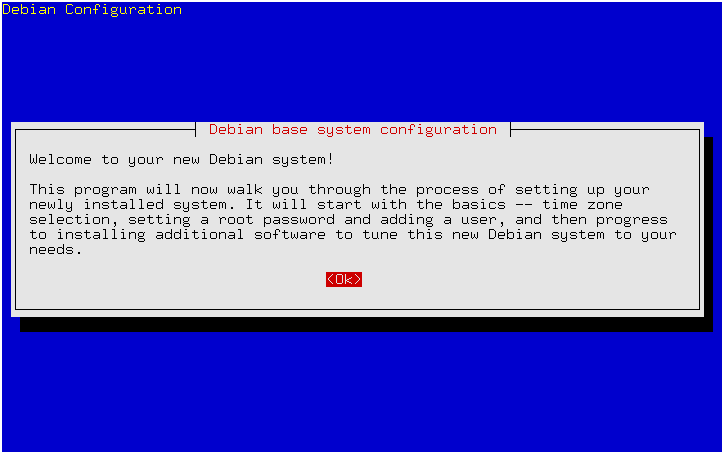
\includegraphics[height=6cm]{201-bc-intro}}
  \only<2>{
  \begin{itemize}
  \item After the reboot base-config is started
    \begin{itemize}
    \item Setup root password
    \item Add a ``normal'' User
    \item Choose installation sources
    \item Select additional packages and tasks
    \end{itemize}
  \item All packages are configured (mostly using debconf)
  \item \alert{This stage of the installation is not part of this talk}
  \end{itemize}
}
}  

\frame[label=summary]{
  \frametitle{Summary: advantages and features of d-i}
   \begin{block}<1->{Advantages}
    \begin{itemize}
    \item Easy default installs
      \begin{itemize}
      \item ``Wizard style'' guided installation
      \item Reasonable default options
      \item Minimum of questions asked
      \end{itemize}
    \item Possibility of expert installs for fine tuning
    \item Modular design makes additions easy
    \end{itemize}
  \end{block}
  \begin{block}<2->{Normal Linux system, but}
    \begin{itemize}
    \item Very specific purpose
    \item Mainly running only one program
    \item Root filesystem in a RAM disk
    \item Configured to run on almost every hardware
    \end{itemize}
  \end{block}
}

\section[Key components]{D-i key components}
\frame[label=udebs]{
  \frametitle{udebs - installer components}
  \begin{block}<1->{Minimal Debian packages: udebs}
    \begin{itemize}
    \item Normal Debian packages (technically)
    \item Not policy compliant
      \begin{itemize}
      \item No documentation and copyright files
      \item File ending .udeb
      \item Reduced to minimal size
      \end{itemize}
    \end{itemize}
  \end{block}
  \begin{block}<2->{Types of udebs}
    \begin{itemize}
    \item Perform an installation step
      \begin{itemize}
      \item Provide a menu item (Choose language, Install the base system, ...)
      \item Postinst script to perform actions
      \end{itemize}
    \item Contain support files
      \begin{itemize}
      \item Kernel modules
      \item Programs (discover, busybox, ...)
      \item Libraries (full libc, libparted, ...)
      \end{itemize}
    \end{itemize}
  Companion: udpkg - a stripped down dpkg
  \end{block}
}
\frame[label=cdebconf]{
  \frametitle{cdebconf - user input}
  \only<1>{
    \begin{block}{Debconf}
      \begin{itemize}
      \item \alert{All user input uses debconf!}
      \item Reimplementation of debconf in C
      \item Same protocol with some additions
        \begin{itemize}
        \item Progress bars
        \item Error notes
        \end{itemize}
      \item Separation of protocol, storage back-end and front-end
        \begin{itemize}
        \item Preseeding of debconf database for automated installs
        \item In the future possible to have other back-ends (eg. LDAP server)
        \item Different front-ends for different purposes
        \end{itemize}
      \item Standard debconf tools can be used for i18n
      \end{itemize}
    \end{block}
  }
  \only<2>{
    \begin{block}{Priority}
      \begin{itemize}
      \item Each question has its priority (low, medium, high or critical).
      \item D-i runs at a given priority (normally at high).
      \item Questions below the current priority are not shown (default answer).
      \item The priority is dynamically lowered on error (and raised on subsequent success).
      \item Installs at priority critical do currently not work!
      \end{itemize}
    \end{block}
  }
  \only<3>{
    \begin{block}{Front-ends}
      \begin{itemize}
      \item Standard newt front-end
      \item Text front-end
      \item Graphical GTK front-end (inactive)
      \item ...
      \end{itemize}
    \end{block}
  }
  \only<4>{
    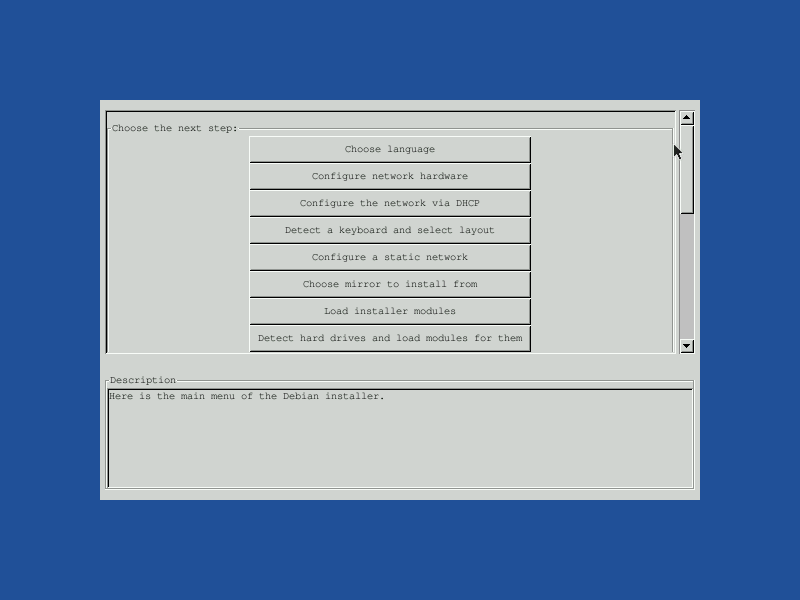
\includegraphics[height=6cm]{main-menu-gtk}

    Screenshot using experimental GTK front-end
  }
}
\frame[label=main-menu]{
  \frametitle{main-menu - Choosing the Next Step}
  \only<1>{
    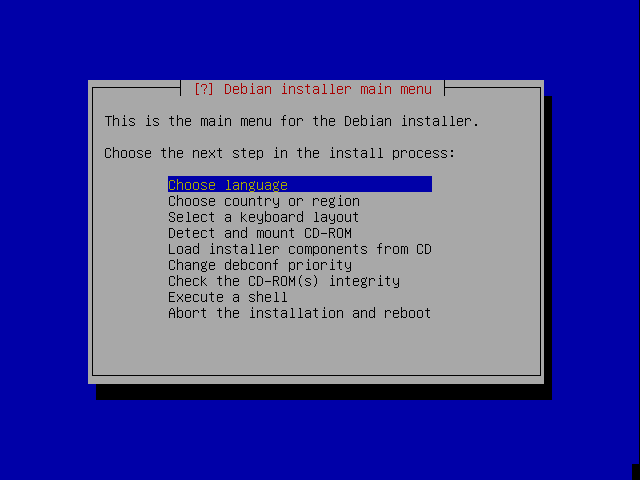
\includegraphics[height=6cm]{003-initial-menu}

    Main-menu after booting the installer.
  }
  \only<2>{
    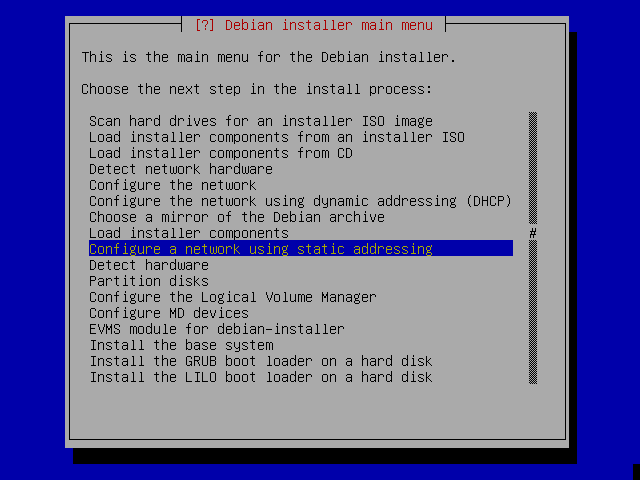
\includegraphics[height=6cm]{020-menu-full}
    
    Full main-menu after loading of additional components.
  }
  \only<3>{
    \begin{itemize}
    \item Central component controlling the installation process
    \item A debconf ``select'' question
    \item \alert{Never shown in default installs (priority medium)!}
    \item More than a menu
      \begin{itemize}
      \item Dynamically adds items as new udebs are installed.
      \item Chooses next action based on menu item number, provides and dependencies.
      \item Calls udpkg to run postinst scripts.
      \end{itemize}
    \end{itemize}
  }
}
\frame[label=coding]{
  \frametitle{Shell and C Code only}
  \begin{block}<1->{Space is very limited}
    \begin{itemize}
    \item No PERL, no Python, no ... (insert your favourite scripting language)
    \item d-i should fit on 2 floppies (kernel and initrd)
    \item d-i should be able to install with minimal RAM (currently approx. 32MB)
    \end{itemize}
  \end{block}
  \begin{block}<2->{Programs either in C or shell (busybox)}
    \begin{itemize}
    \item Shell prefered
    \item Easier to debug and maintain
    \item ``Live changes'' possible
    \item Only stripped down tools from BusyBox
    \item nano as an editor (and pager)
    \item C where shell is not feasible (BusyBox, discover, ...)
    \end{itemize}
  \end{block}
}

\section[udebs]{Interesting udebs}
\frame[label=chooser]{
  \frametitle{country-/language-/kbd-chooser}
  \framesubtitle{\textbf{Packages: languagechooser, countrychooser, kbd-chooser}}
  \only<1>{
    \begin{block}{languagechooser lists all available translations}
      \begin{itemize}
      \item \alert{languagechooser is the first screen shown on ordinary d-i installs!}
      \item Everything shown after this should continue localized
      \item Language choice affects defaults for country and keyboard selection
      \end{itemize}
    \end{block}
  }
  \only<2>{
    \begin{block}{countrychooser lists countries}
      \begin{itemize}
      \item Small list of countries based on language
      \item Full list on second screen
      \item Choice affects default locale
      \item Tricky to not set an unsupported locale (eg. de\_ZH = German as spoken in China)
      \item The choice of country names can be very controversial and political (eg. Taiwan).
      \end{itemize}
    \end{block}
    \begin{block}{kbd-chooser lists available keyboard layouts and types}
      \begin{itemize}
      \item The default option is based on the answers to the language and country questions.
      \end{itemize}
    \end{block}
  }
  \only<3>{
    \begin{columns}
      \column{4.5cm}
      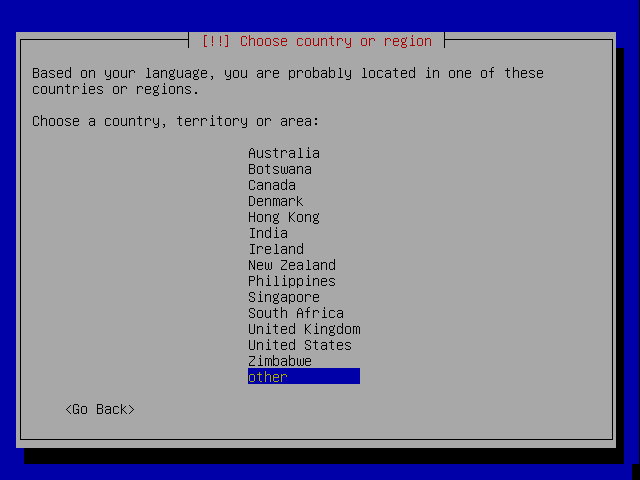
\includegraphics[width=4.4cm]{005-region}
      \column{4.5cm}
      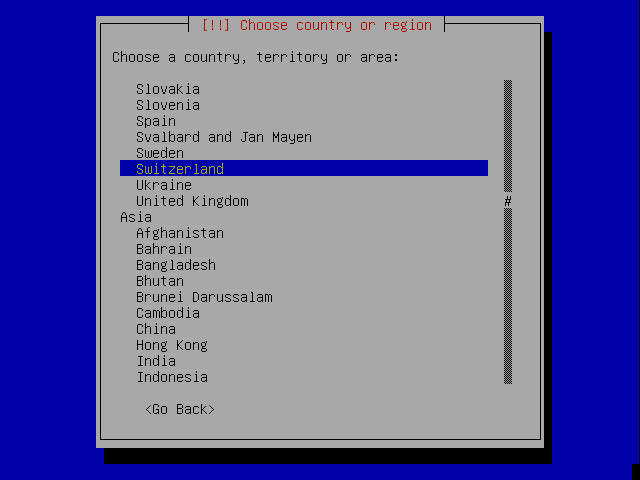
\includegraphics[width=4.4cm]{006-region-other}
    \end{columns}

    First and second countrychooser screen
  }
}
\frame[label=ddetect]{
  \frametitle{Hardware detection}
  \framesubtitle{\textbf{Packages: discover1, discover1-data, ddetect (ethdetect, hw-detect, hw-detect-full)}}
  \only<1>{
    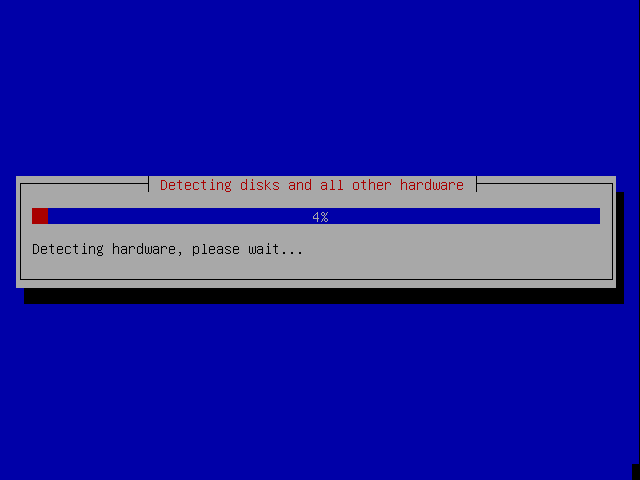
\includegraphics[height=6cm]{047-hw-detect}
    
    Hardwre detection in progress...
  }
  \only<2-3>{
    \begin{block}<2-3>{Hardware detection with discover}
      \begin{itemize}
      \item Currently based on discover 1.6 
      \item Chooses kernel modules based on PCI IDs
      \item Runs 3 times 
        \begin{itemize}
        \item ethernet card
        \item CD drive
        \item full hardware (hard disk)
        \end{itemize}
      \end{itemize}
    \end{block}
    \begin{block}<3>{Hardware database}
      \begin{itemize}
      \item Constantly growing
      \item Needs updates for new hardware
      \item No fully automated source exists
      \item Updated from bug and installation reports
      \end{itemize}
    \end{block}
  }
  \only<4>{
    \begin{block}{Some things are hardcoded}
      \begin{itemize}
      \item Modules not connect to hardware (iso9660, ide-probe, ...)
      \item Most IDE device support (was 1 module in the past)
      \end{itemize}
    \end{block}
  }
}
\frame[label=anna]{
  \frametitle{anna and retrievers}
  \framesubtitle{\textbf{Packages: anna, \{net,cdrom,floppy\}-retriever}}
  \only<1>{
    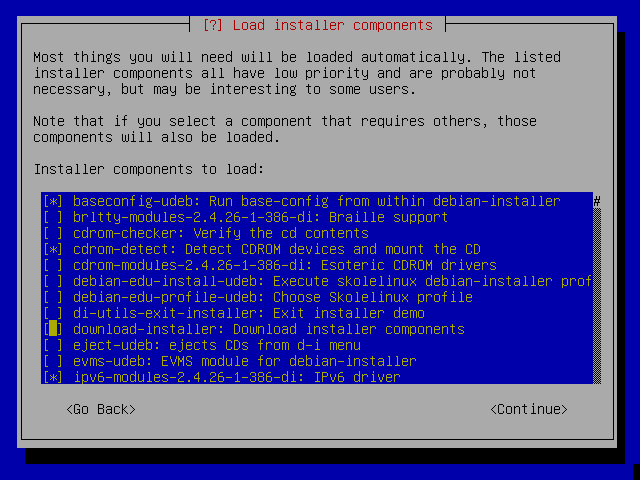
\includegraphics[height=6cm]{018-comps-choose}
    
    anna's not nearly apt, but for Debian installer, it will do
  }
  \only<2-3>{
    \begin{block}<2->{system to download/install additional components}
      \begin{itemize}
      \item installs all udebs with priority greater than standard
      \item resolves dependencies
      \item changes to the list of selected udebs are possible at debconf priority smaller than medium
      \end{itemize}
    \end{block}
    \begin{block}<3->{udebs are downloaded/installed by retrievers}
      \begin{itemize}
      \item net-retriever to download from a Debian mirror
      \item cdrom-retriever to install from a mounted CD-ROM (or loop mounted iso-image)
      \item floppy-retriever to install some udebs from floppy and rerun anna afterwards
      \end{itemize}
    \end{block}
  }
}
\frame[label=partman]{
  \frametitle{partman - partitioning and mount points}
  \framesubtitle{\textbf{Packages: partman-*, mdcfg, lvmcfg}}
  \only<1>{
    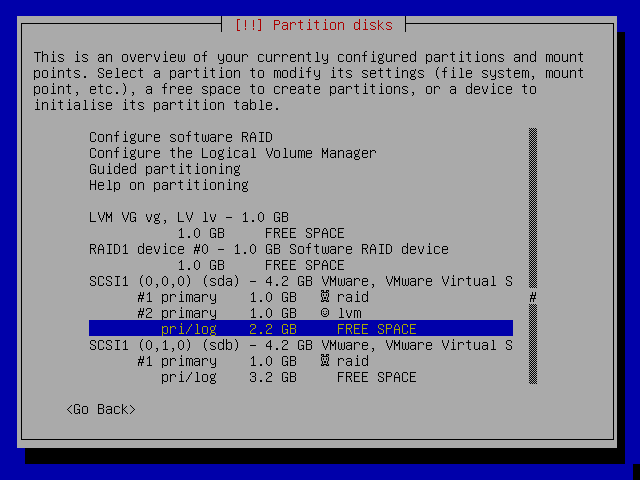
\includegraphics[height=6cm]{058-part-destinations}

    Partman's main screen
  }
  \only<2-3>{
    \begin{block}<2-3>{Features}
      \begin{itemize}
      \item Multiple filesystem support:
        \begin{itemize}
        \item ext2/3
        \item reiserfs
        \item jfs
        \item xfs
        \end{itemize}
      \item Support for LVM and software RAID
      \item Automatic and manual partitioning
      \item Based on libparted
      \end{itemize}
    \end{block}
    \begin{block}<3>{Split into several small udebs:}
      \begin{itemize}
      \item One for each supported filesystem
      \item Simple to add support for new filesystems
      \item Additional udebs for architecture support
      \item Any addition can be implemented in it's own udeb
      \end{itemize}
    \end{block}
  }
  \only<4>{
    \begin{block}{``Client/Server'' architecture}
      \begin{itemize}
      \item Server written in C performs actions using libparted
      \item Clients written in Shell send commands over FIFOs
      \end{itemize}
    \end{block}
    Partman would be a topic for a talk on it's own.
  }
}
\frame[label=bootloader]{
  \frametitle{Boot Loader Installers}
  \framesubtitle{\textbf{Packages: \{aboot, delo, grub, lilo, palo, yaboot, ...\}-installer, os-prober, nobootloader}}
  \only<1>{
    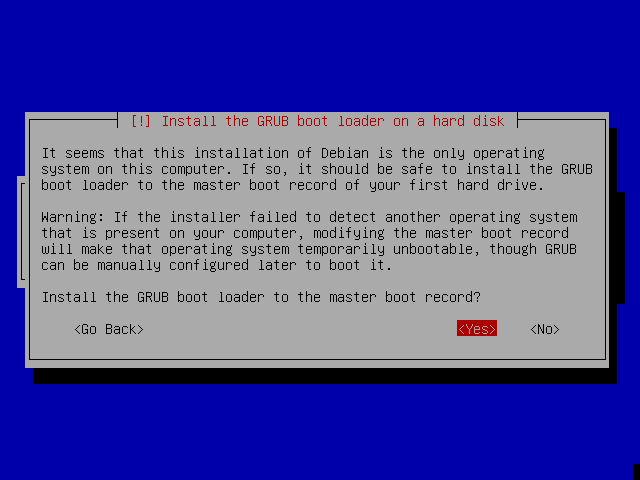
\includegraphics[height=6cm]{096-grub-install-mbr}
    
    grub-installer asking where to install grub
  }
  \only<2>{
    \begin{itemize}
    \item Separate small udebs to install the boot loader
    \item Grub currently default on i386
    \item Special os-prober udeb to detect other operating systems and to offer multiboot
    \item nobootloader udeb to skip bootloader installation on systems that don't need a boot loader
    \end{itemize}
  }
}

\section{Further Information}
\frame[label=images]{
  \frametitle{Available images}
  \only<1-3>{
    There is sometimes confusion about the content of the different d-i images.
    \begin{block}<2-3>{ISO images}
      http://cdimage.debian.org/pub/cdimage-testing/
      \begin{itemize}
      \item Netinst image: all udebs and base system debs
      \item Businesscard image: only udebs, downloads base system from mirror
      \item sid\_d-i: udebs from sid, base system from Sarge
      \item sarge\_d-i: udebs and base system debs from Sarge
      \item daily: currently symlink to sarge\_d-i
      \end{itemize}
    \end{block}
    \begin{block}<3>{other Images}
      \begin{itemize}
      \item Daily builds: http://www.debian.org/devel/debian-installer/ports-status
      \item betas: dists/testing/main/installer-\{arch\} on any Debian mirror
      \end{itemize}
    \end{block}
  }
  \only<4>{
    How to test?
    \begin{enumerate}
    \item Latest beta or release candidate
    \item Check if errors are still present in latest sarge\_d-i or sid\_d-i images.
    \item \alert{Fill out installation report!}
    \end{enumerate}
  }
}
\frame[label=svn]{
  \frametitle{D-i Subversion Repository}
  \begin{itemize}
  \item d-i is hosted on Alioth (project: d-i)
  \item uses Subversion for source control
  \item Anonymous checkout: \texttt{svn co svn://svn.debian.org:3691/d-i/trunk debian-installer}
  \item Source snapshots available on http://d-i.alioth.debian.org/
  \item Sorry, currently no viewcvs access.
    \begin{itemize}
    \item Locking problems with SVN repository on Alioth
    \end{itemize}
  \item \alert{Easy to get an Alioth account and participate}
  \end{itemize}
}
\frame[label=contact]{
  \frametitle{Documentation and Contact Info}
  \begin{itemize}
  \item trunk/installer/doc in SVN
    \begin{itemize}
    \item Installation manual (work in progress)
    \item (Some) documentation about d-i
    \end{itemize}
  \item debian-boot@lists.debian.org
  \item \#debian-boot on irc.freenode.net
  \item http://www.debian.org/devel/debian-installer
  \item http://wiki.debian.net/?DebianInstaller
  \end{itemize}
}

\section{Discussion}
\frame[label=discussion]{
  \frametitle{Discussion}
  \alert{It's your turn now!}
  
  /me hopes he will know at least some of the answers.
}

\appendix
\section{\appendixname}
\frame{\tableofcontents}

\subsection{Additional udebs}
\frame[label=netcfg]{
  \frametitle{netcfg}
  \framesubtitle{\textbf{Packages: netcfg, netcfg-dhcp, netcfg-static}}
  \begin{itemize}
  \item Network configuration for d-i and installed system
  \item Trys DHCP first
  \item Offers manual configuration if no DHCP server replies
  \end{itemize}
}
\frame[label=libd-i]{
  \frametitle{libdebian-installer}
  \framesubtitle{\textbf{Package: libdebian-installer4, libdebian-installer-extra4}}
  \begin{itemize}
  \item Common C functions
    \begin{itemize}
    \item Package parser
    \item Logging
    \item ...
    \end{itemize}
  \end{itemize}
}

\frame[label=base-installer]{
  \frametitle{base-installer}
  \framesubtitle{\textbf{Packages: base-installer, debootstrap-udeb}}
  \only<1>{
    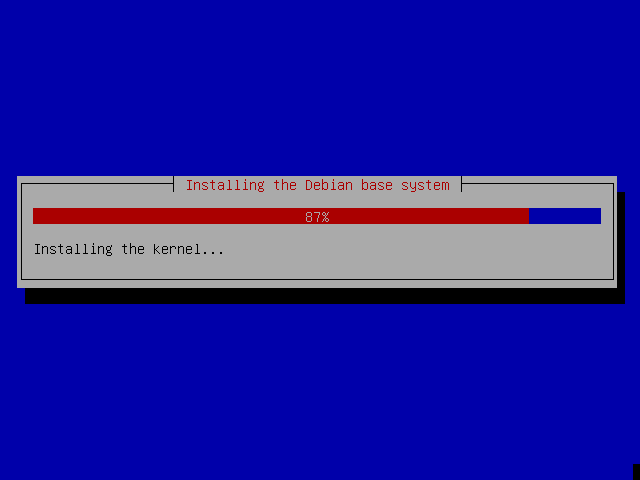
\includegraphics[height=6cm]{095-kernel-install}
    
    base-installer installing the kernel
  }
  \only<2>{
    \begin{itemize}
    \item Installs base-system (by calling debootstrap)
    \item Installs extra packages (registered by apt-install)
    \item Chooses and installs kernel
    \end{itemize}
  }
}

\subsection{Custom Images}
\frame[label=kernel-wedge]{
  \frametitle{kernel-wedge - industrial strength kernel splitting tool}
  \framesubtitle{\textbf{Package: kernel-wedge}}
  \begin{itemize}
  \item Splits Debian kernel package into small udebs
  \item Lists of modules per udeb
  \item Predefined lists in linux-kernel-di-{arch}
  \end{itemize}
http://d-i.alioth.debian.org/svn/debian-installer/installer/doc/custom-kernel.txt
}
\frame[label=build]{
  \frametitle{How to Build Custom Images}
  \begin{block}<1->{d-i images}
    \begin{itemize}
    \item Directory installer/build in SVN
    \item Build system based on make
    \item Only builds initrds and kernel image
    \item Run make without target to list useful targets
    \end{itemize}
  \end{block}
  \begin{block}<2->{debian-cd}
    \begin{itemize}
    \item Builds ISO images
    \item Difficult to install, needs Debian mirror
    \end{itemize}
  \end{block}
  \begin{block}<3->{Hacks}
    \begin{itemize}
    \item Modify ISO image built with debian-cd
    \item Some hacks are documented in the d-i wiki.
    \end{itemize}
  \end{block}
}

\subsection{Questions}
\frame[label=graphical]{
  \frametitle{Why is there no graphical front-end?}
  \begin{itemize}
  \item We want to do it right.
    \begin{itemize}
    \item Good graphical user interface
    \item Comparable to other graphical installers
    \end{itemize}
  \item Current GTK front-end has the same UI as the newt front-end.
  \item Some ideas to solve the UI problem exist.
  \item Nobody is working on it.
  \end{itemize}
}

\end{document}
